\documentclass[sigconf, authordraft]{acmart}

\usepackage{booktabs} % For formal tables


% Copyright
%\setcopyright{none}
%\setcopyright{acmcopyright}
%\setcopyright{acmlicensed}
\setcopyright{rightsretained}
%\setcopyright{usgov}
%\setcopyright{usgovmixed}
%\setcopyright{cagov}
%\setcopyright{cagovmixed}


% DOI
%\acmDOI{10.475/123_4}

% ISBN
%\acmISBN{123-4567-24-567/08/06}

%Conference
\acmConference[GECCO '18]{the Genetic and Evolutionary Computation Conference 2018}{July 15--19, 2018}{Kyoto, Japan}
\acmYear{2018}
\copyrightyear{2018}

\begin{document}
\title{Structure of a Well-Known Modularity-Inducing Problem Domain} %Temporary running title
\titlenote{Produces the permission block, and
  copyright information}

\author{Author One}
\affiliation{%
  \institution{Institution}
  \streetaddress{Omitted}
  \city{Omitted}
  \state{Omitted}
  \postcode{1234}
}
\email{abc@def}

\author{Author Two}
\affiliation{%
  \institution{Institution}
  \streetaddress{Omitted}
  \city{Omitted}
  \state{Omitted}
  \postcode{1234}
}
\email{def@def}

\author{Author Three}
\affiliation{%
  \institution{Institution}
  \streetaddress{Omitted}
  \city{Omitted}
  \state{Omitted}
  \postcode{1234}
}
\email{ghi@def}



% The default list of authors is too long for headers.
\renewcommand{\shortauthors}{Author One et al.}


\begin{abstract}
A long-standing biological question is how organisms can quickly adapt themselves to new environments that are constantly changing, which is called evolvability. A key aspect to understand evolvability is to know the origin of modularity. In the computational biology, one prevalent theory argues that gene specialization drives modularity. Our experiments indicated that there existed an inconsistency between this theory and observations in biology, regarding the dominant status of modular structures on evolvability. Subsequent experiments also indicated that networks with high fitness could be converted into modular structures by removing inter-module connections while their performance improved. Further experiments demonstrated that more fluctuant evolving landscape can also promote a higher level of network modularity, compared with a more fixed landscape in which networks search for optimums. We also showed that more modular structures may require fewer connections. Therefore, modular networks may evolve towards structures that require a fewer total number of edges.
\end{abstract}

%
% The code below should be generated by the tool at
% http://dl.acm.org/ccs.cfm
% Please copy and paste the code instead of the example below.
%
\begin{CCSXML}
<ccs2012>
 <concept>
  <concept_id>10010520.10010553.10010562</concept_id>
  <concept_desc>Computer systems organization~Embedded systems</concept_desc>
  <concept_significance>500</concept_significance>
 </concept>
 <concept>
  <concept_id>10010520.10010575.10010755</concept_id>
  <concept_desc>Computer systems organization~Redundancy</concept_desc>
  <concept_significance>300</concept_significance>
 </concept>
 <concept>
  <concept_id>10010520.10010553.10010554</concept_id>
  <concept_desc>Computer systems organization~Robotics</concept_desc>
  <concept_significance>100</concept_significance>
 </concept>
 <concept>
  <concept_id>10003033.10003083.10003095</concept_id>
  <concept_desc>Networks~Network reliability</concept_desc>
  <concept_significance>100</concept_significance>
 </concept>
</ccs2012>
\end{CCSXML}

\ccsdesc[500]{Computer systems organization~Embedded systems}
\ccsdesc[300]{Computer systems organization~Redundancy}
\ccsdesc{Computer systems organization~Robotics}
\ccsdesc[100]{Networks~Network reliability}


\keywords{ACM proceedings, \LaTeX, text tagging}


\maketitle

% Here comes the main part of the paper
\section{Introduction}

\section{Background}
Figure \ref{fig:network-example} demonstrates examples of non-modular and modular networks.  
%\begin{figure}[h!]
%	\centering
%	\begin{subfigure}[b]{0.45\linewidth}
%		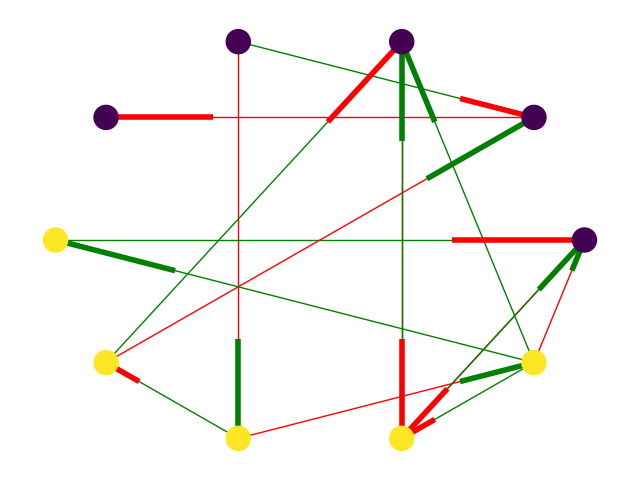
\includegraphics[width=\linewidth]{non-modular-example.png}
%		\caption{A non-modular example}
%	\end{subfigure}
%	\begin{subfigure}[b]{0.45\linewidth}
%		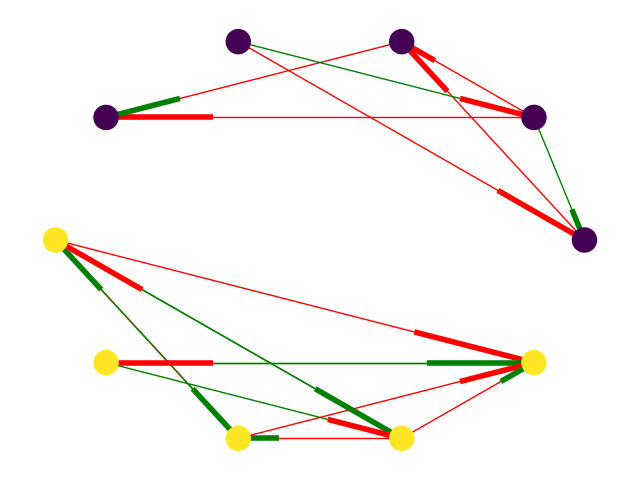
\includegraphics[width=\linewidth]{modular-example.png}
%		\caption{A modular example}
%	\end{subfigure}
%	\caption{Non-modular and modular networks}
%	\label{fig:network-example}
%\end{figure}
In the inception phase of this project, we utilized the Louvain heuristics to compute the partition of the network vertices in order to maximize the modularity of the given graph \cite{blondel2008fast}. We applied the tournament selection scheme with the tournament size being three and the elitism mechanism with ten elites in every generation. As a result of this setting, the partition of the gene regulatory networks by the Louvain heuristics demonstrated a very low modularity score. As Figure \ref{fig:early-modularity-not-work} indicates where the green line represents the generation to introduce specialization, by simulating the work in \cite{espinosa2010specialization}, we had expected there would be a spike after gene specialization on modularity. Nevertheless, we observed a modularity decrease as a result after gene specialization. 
\begin{figure}[h!]
	\centering
	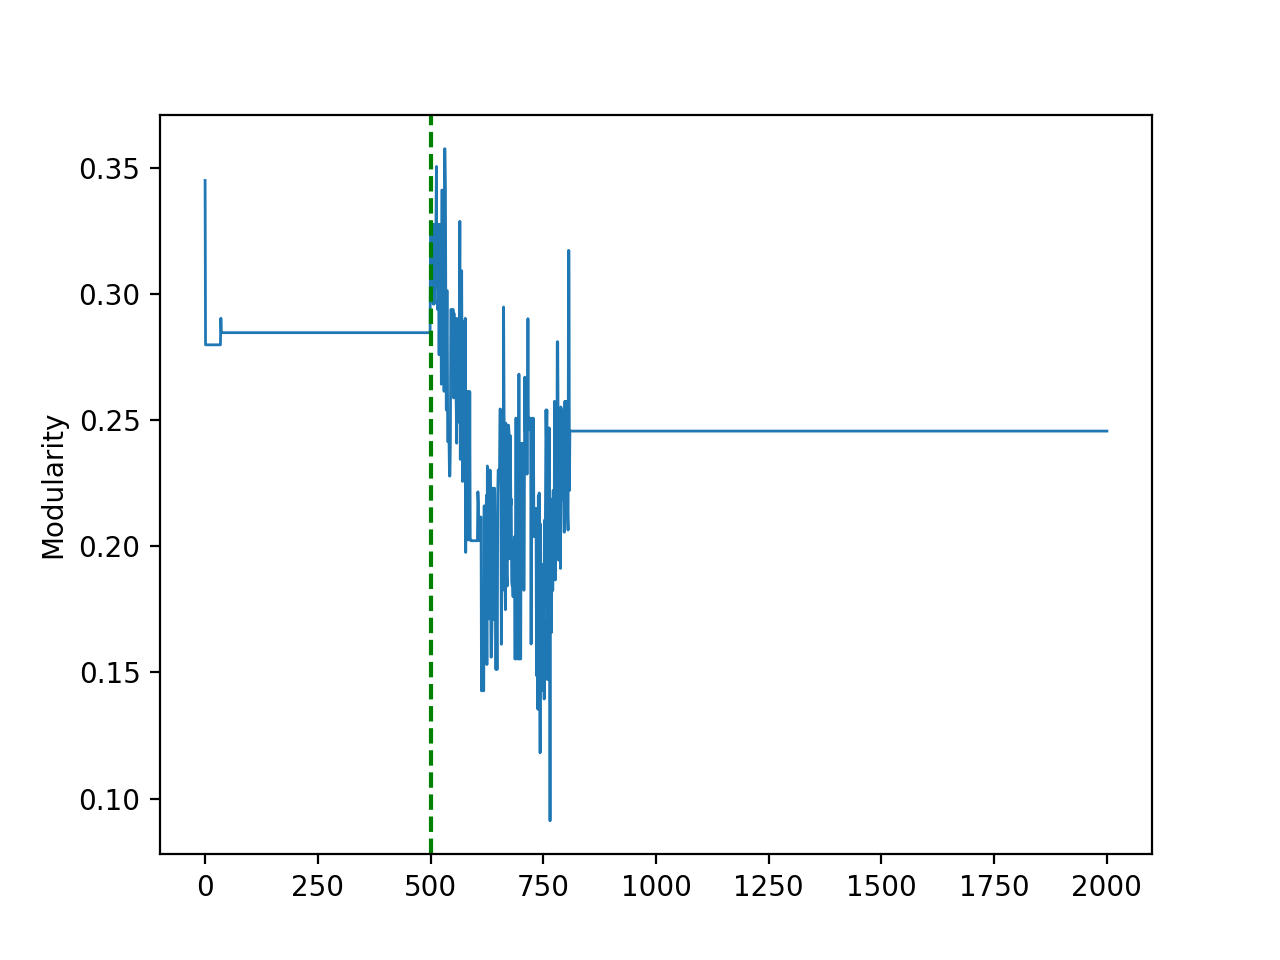
\includegraphics[width=\linewidth]{early-elitism-not-work.png}
	\caption{Modularity went worse after gene specialization}
	\label{fig:early-modularity-not-work}
\end{figure}
\begin{figure}[h!]
	\centering
	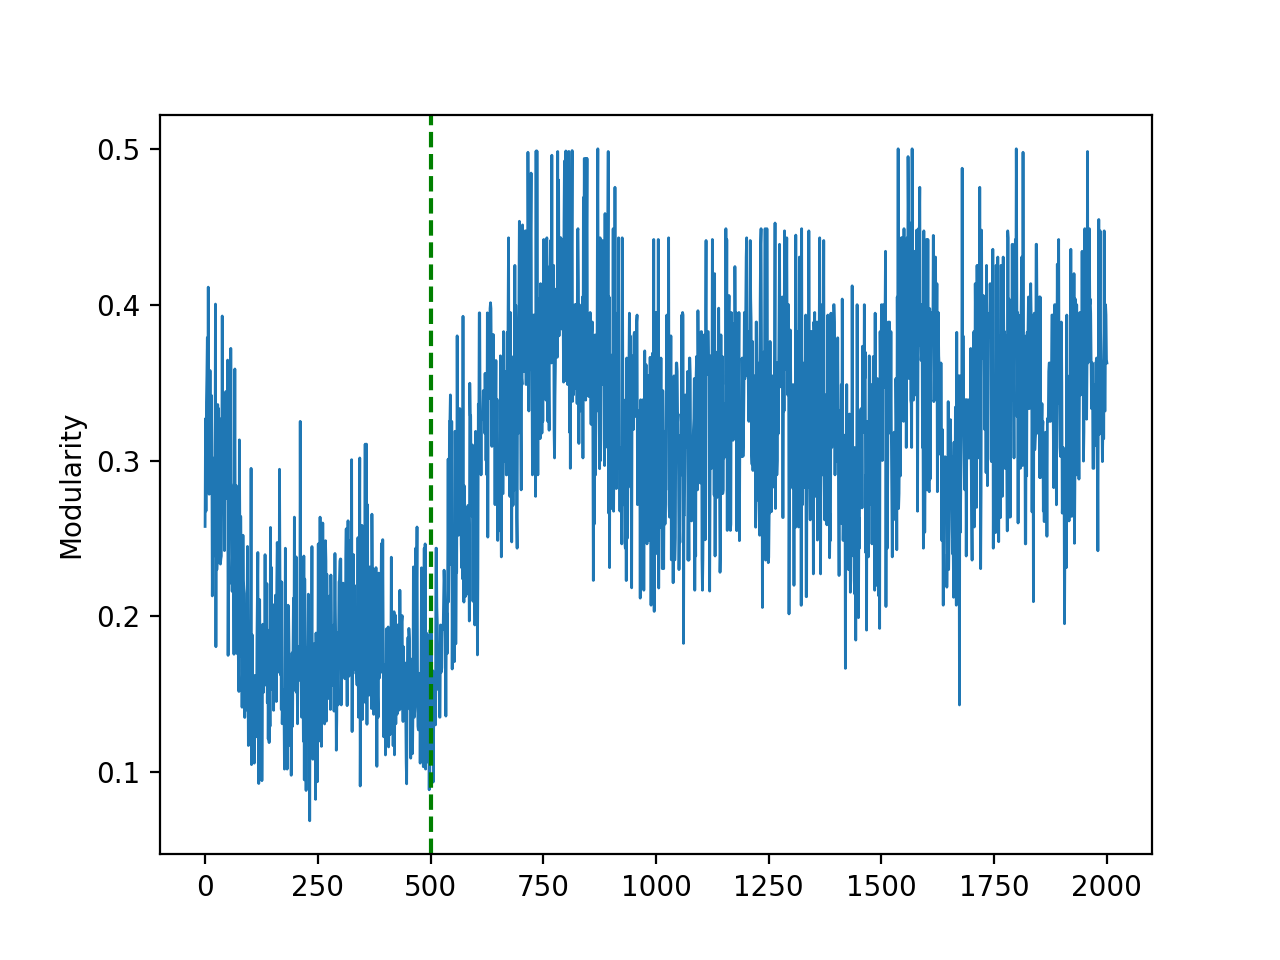
\includegraphics[width=\linewidth]{modularity-worked.png}
	\caption{Modularity emerged after gene specialization without elitism}
	\label{fig:modularity-worked-without-elitism}
\end{figure}
In order to understand this puzzling phenomenon, we removed the elitism mechanism and changed the tournament to proportional selection scheme. In consequence, we eliminated the deviant phenomenon as Figure \ref{fig:modularity-worked-without-elitism} indicates. Therefore, we hypothesized that the elitism mechanism or the tournament selection scheme hamper the evolutionary process on evolving out modular structures. 


\section{Methods}
This is where we describe what we're going to do. As discussed previously, 
we don't mention symmetry or noisy evaluation in this paper, nor do we cover 
hotspots, diploidy or dominance.

What we do work with is a basic GA with mutation as per previous work, and cross
over. The variations are:

Espinosa Soto vs Larson fitness function
Fitness proportionate (roulette) selection vs tournament (maybe a couple of different tournament sizes)

We may end up merging this with the experiments section

We utilize genetic algorithms as our evolutionary simulation tools. The gene regulatory network that we used in this paper was originally proposed by Wagner \cite{wagner1996does} and customized by Espinosa-Soto and Wagner \cite{espinosa2010specialization} as well as Larson et al. \cite{larson2016recombination}. 

All simulation code was implemented in Java 1.8.0 and Python 2.7.10. They are all publicly available at https://github.com/xxxxxxxxxx. Modularity was evaluated using the NetworkX package with the community API \cite{hagberg2008exploring}. All the generated data can be downloaded at: https://drive.google.com/file/xxxxxxxxxxxxxxxxxx. 

\subsection{Model}
Cells in an organism display heterogeneity in functionalities and morphologies, while they contain the same set of genes. In other words, cells interpret the same genetic material in different ways so that their behaviours and structures vary. These distinct interpretations are due to the regulation via the activation and repression of genes \cite{wagner1996does}. In brief, effects of different genes are not mutually independent. A protein that is generated by a gene may activate or repress other genes. A gene regulatory network can be a mathematical directed graph to express these relationships of genes in an organism \cite{wagner1996does}. Specifically, genes can have two different patterns, namely activation and repression. The term "gene activity pattern" is adopted to represent the activeness status of the entire set of genes. Different gene activity patterns mean the distinct cellular functions and forms \cite{espinosa2010specialization}. 

We re-constructed the model that was utilized in the work done by Espinosa-Soto and Wagner, which is a model to represent a gene regulatory network \cite{espinosa2010specialization}. In this model, a gene regulatory network with $N$ genes will be in the form of an adjacency matrix $A = a_{ji}$, which acts as a genotype of an individual. Each entry $a_{ji}$ is restricted to be either 1, 0 or -1, which represents an activation, absence or repression interaction from gene $j$ to gene $i$, respectively. The gene activity pattern of this network at time $t$ can be expressed as a Boolean row vector $s_{t} = [s_{t}^0,...,s_{t}^{N-1}]$. A certain gene $i$ can either be active ($s_t^i=1$) or inactive ($s_t^i=-1$). The transition of state activity is modelled by the equation below
\begin{equation}
s_{t+\tau}=\sigma[\sum_{j=1}^{N}a_{ji}s_t^j]
\end{equation}
where $\sigma(x)$ equals 1 if $x>0$ and is 0 otherwise. 

\subsection{Fitness}
The fitness here evaluates the likelihood that an attractor is obtained when facing perturbations \cite{espinosa2010specialization}. In other words, Espinosa-Soto and Wagner imposed a bias of robustness on their gene regulatory network models in order to indirectly select modular networks. This is because modular networks can limit perturbations in a module so that the overall structure will not be heavily affected \cite{aderems2005systems}. That is, more modular networks are more robust. 

There are two or more stages in their experiments on discovering the conditions under which modularity starts emerging. In the first stage, gene regulatory networks are evolved under selective pressure towards regulating a particular gene activity pattern, while facing some perturbations. The original gene activity pattern before perturbation is called a target. In the second and further stages, networks are evolved under selective pressure to regulate new gene activity patterns, while preserving the ability to regulate the old patterns. In the particular case where there were two gene activity patterns, the first stage lasted for 500 generations and the second took another 1500 generations. 

The perturbations of targets are randomly generated in every generation when evaluating the fitness of gene regulatory networks. In Espinosa-Soto and Wagner's experiments, a network would face 500 perturbations comprising different corrupted versions of gene activity patterns. Each gene will have a probability of 0.15 to be perturbed into its opposite activity. A further study was conducted to explore a sufficient number of perturbations in order to shorten the computational time while maintaining a similar eventual improved modularity. It was concluded that 75 or 100 perturbations would lead to the noteworthy emergence of modularity \cite{totten2015exploring}. Therefore, 75 perturbations are undertaken for evaluating the fitness of each gene regulatory network in order to reduce the running time. 

Larson et al. applied another approach for evaluating the fitness of networks \cite{larson2016recombination}. They generated a static set of perturbations at the beginning and utilised this same set of corrupted targets whenever network fitness was calculated. This method converts the original stochastic fitness evaluation into a deterministic one. That is, the evolutionary landscape of individuals under this fitness evaluation will remain unchanged in each generation. On contrast, Espinosa-Soto and Wagner's fitness evaluation will lead to the evolutionary landscape to shift every generation. 

The fitness value of a gene regulatory network reflects its robustness in recovering from various perturbations. The error function compares an attractor of the network dynamics to the original gene activity pattern. That is, a successful network is able to regulate a corrupted pattern to its initial form. Then, the Hamming Distance G between the attractor and the original pattern was calculated. Previous experiments indicated that it normally took fewer than 20 transitions to reach the attractor \cite{wagner1996does}. Thus, non-stable attractors are assumed to be those gene regulatory networks that take more than 20 steps to attain the stability, or are cyclically stable. They are treated to have a maximum Hamming distance $D_{max}$. This is followed by a calculation of the contribution from each perturbation attractor to the fitness, which is defined as a developmental trajectory $\gamma=(1-D/D_{max})^5$ \cite{espinosa2010specialization}. Afterwards, this process is repeated to determine 75 $\gamma_{i}$, $1 \leq i \leq 75$. Finally, the fitness of a network is calculated as
\begin{equation}
f(g)=1-e^{-3g}
\end{equation}
where $g$ represents the artimetic mean of the sum of all $\gamma_{i}$ \cite{espinosa2010specialization}. As to cases where there are more than one gene activity patterns, the arithmetic mean of $f(g)$ for all the patterns was take. Consequently, a gene regulatory network with a high fitness is able to lead to different attractors matching different targets. 

\subsection{Evolutionary Simulations}
Espinosa-Soto and Wagner imposed a bias towards low-density gene regulatory networks in mutation \cite{espinosa2010specialization}. A node in the network has a probability $\mu=0.05$ to mutate every generation, and it either can lose or gain an interaction. The probability for a node to lose an interaction can be calculated as
\begin{equation}
p(u)=\frac{4r_{u}}{4r_{u} + N - r_{u}}
\end{equation}

where $N$ is the number of gene nodes in a gene regulatory network, and $r_{u}$ equals to the number of regulators of gene $u$ \cite{espinosa2010specialization}. That is, the number of genes that exert effects on gene $u$. In contrast, the probability for a gene $u$ to obtain an interaction is defined to be $1-p(u)$. That is, it can keep the sparseness of the network, which computational biology research suggests is necessary for the emergence of modularity. 

Espinosa-Soto and Wagner did not apply a crossover mechanism in their simulation \cite{espinosa2010specialization}. In the reconstructed model by Larson et al., they limited crossover to nine possible partition locations of a 10-node network, corresponding to nine possible rows for splitting the adjacency matrix of a network horizontally \cite{larson2016recombination}. When two matrices $A_{1}$ and $A_{2}$ are selected for crossover at index $i$, matrices of their children will be produced as \\ \\
$C_{1}[0: i-1, :] = A_{1}[0: i-1, :]\\
C_{1}[i: 9, :] = A_{2}[i: 9, :]\\
C_{2}[0: i-1, :] = A_{2}[0: i-1, :]\\
C_{2}[i: 9, :] = A_{1}[i: 9, :]\\$

However, this horizotal crossover may not only make the parental networks exchange modular clusters, but also exchange some interactions between the two modules. This may corrupt modularity. In contrast, we use a crossover mechanism that swaps interactions between modules in a gene regulatory network with connections between modules in another network. Compared with the crossover mechanism of Larson et al., this approach, as Figure X illustrates, will better preserve the community structure (Wilcoxon signed-rank test; $p<0.0372$). 

\subsection{Modularity Metric}
We adopted the Q scoring system to quantify modularity in a network based on the algorithm proposed by Newman \cite{newman2004finding}. Briefly, this approach is defined as the difference between the ratio of the number of edges in the network connecting nodes within a module over the number of all the edges, and the same quantity when assigning the nodes into the same modules yet edges are assumed to be randomly connected in the network \cite{kashtan2005spontaneous}. Formally, $Q$ is calculated as 
\begin{equation}
Q = \sum_{i}^{K}[\frac{l_i}{L} - (\frac{d_i}{2L})^2]
\end{equation}
where $i$ represents one of the $K$ potential modules within a network, $L$ is the total number of connections in a network, $l_i$ stands for the number of interactions in the module $i$, and $d_i$ is the sum of degrees of all the nodes in module $i$ \cite{espinosa2010specialization}. In other words, $Q$ considers the two ratios of both intra-module connection density and inter-module connection density \cite{newman2004finding}. A network that is considered to be good on modularity must consist of as many within-module edges and as few inter-module edges as possible. However, it will result in $Q=0$ if all the nodes are partitioned into the same module. 

The value $Q$ will sit in the range of $\left.[-\frac{1}{2}, 1\right.)$. Nodes in the gene regulatory network are partitioned into different groups according to their regulating gene activity patterns. 





\section{Experiments}
Gene activity patterns and the essential parameters of our evolutionary simulations are provided in the form of Tables 4.1 and 4.2 in order to facilitate repeatability of these experiments. The detailed explanations of these parameters are given after Table 4.2. Overall, only the elite number and the tournament size will be specified in each experiment, since only those may vary in different experiments. All the other parameters are specified in Table 4.1 and 4.2 are consistent in the experiments. 
\vspace*{-12 pt}
\begin{table}[h]
	\centering
	\caption{Table to test captions and labels}
	\label{table:4.1}
	\begin{tabular}{|c | c|} 
		\hline
		Gene Activity Pattern & Generation to Add a New Pattern \\ [0.5ex] 
		\hline
		1, -1, 1, -1, 1, -1, 1, -1, 1, -1 & 0 \\ 
		\hline
		1, -1, 1, -1, 1, 1, -1, 1, -1, 1 & 500 \\
		\hline
	\end{tabular}
\end{table}

\vspace*{-19.5 pt}
\begin{table}[h]
	\centering
	\caption{Parameters of the evolutionary simulation}
	\label{table:4.2}
	\begin{tabular}{|c | c | c |} 
		\hline
		Edge Size & Perturbation Number & Perturbation Rate \\
		\hline
		20 & 75 & 0.15 \\
		\hline
		Mutation Rate & Population Size & Tournament Size \\
		\hline
		0.05 & 100 & Proportional \\
		\hline
		Reproduction Rate & Maximum Generation & Elite Number \\
		\hline
		0.9 & 2000 & 0 or 10 \\
		\hline
	\end{tabular}
\end{table}

\begin{table}[!htbp]
	\centering
	\caption{Explanations of simulation parameters}
	\label{table:4.3}
	\begin{tabular}{|p{0.3\linewidth} | p{0.7\linewidth}|}
		\hline
		Gene Activity Patterns & the patterns that are perturbed, and towards which gene regulatory networks evolve. \\
		\hline
		Generations to add a new pattern & the generations to add new gene activity patterns towards which networks evolve. \\
		\hline
		Edge Size & the initial number of edges in the original gene regulatory networks. \\
		\hline
		Perturbation Number & the number of corrupted versions of each gene activity pattern. \\
		\hline
		Perturbation Rate & the expectation of the number of corrupted genes in a pattern. \\
		\hline
		Mutation Rate & the probability of a gene node to gain or lose an interaction in a network. \\
		\hline
		Population Size & the number of individuals in the population in every generation. \\
		\hline
		Tournament Size & the size of the tournament selection; where tournament selection is used, the size of the tournament; where proportional sections is used, it is annotated as "proportional". \\
		\hline
		Reproduction Rate & the proportion of children reproduced over the entire population. Any vacancy will be filled by the tournament scheme selecting individuals from the previous generation. \\
		\hline
		Maximum generation & the generation when the simulation will terminate after reaching it. \\
		\hline
	\end{tabular}
\end{table}

\subsection{Diagonal Crossover Mechanism Promotes Modularity}
I simulated 40 independent evolutions for the development with no crossover and with each of the two crossover mechanisms, namely horizontal crossover and diagonal crossover, respectively. None of these simulations applied elitism. Overall, the diagonal crossover mechanism performed better than no crossover and the horizontal crossover, regarding both regulatory performance and modularity emergence, as Tables 3.1 and 3.2 indicate.

The Boolean model that I have utilised to simulate biological networks was originally proposed by Wagner in his study on "epigenetic stability" \cite{wagner1996does}. His work indicated that random recombination made no difference for the evolution of stability, which may be due to the freeness of random recombination on choosing locations to undertake crossover. This can corrupt the modular structures in biological networks.

Conversely, my experimental results suggested that proper recombination methods can contribute to the evolvability of organisms. The diagonal crossover proposed in this report is able to preserve underlying network modules. Although the crossover mechanism utilised by Larson et al. did not preserve community structures as well as diagonal crossover, its partitioning is still based on a network-like structure. This can be the reason why both of these two crossover mechanisms could help in obtaining modularity, with diagonal crossover better than horizontal crossover. Meanwhile, different combinations of parental traits can increase the diversity of the population so that the evolution can be more exploratory.

\subsection{Greed Hampers Modularity}
\subsubsection{Proportional Exceeds Tournament Selection on Generating Modularity}~\\
We simulated 
\subsubsection{Elitism Hampers Modularity}~\\
We simulated 40 evolutionary trials with 10 elites and without any elites. That was 80 trials in total. The experimental results indicate that elitism will hamper both the networks' regulatory capabilities and modularity emergence, as shown in Table 3.3 and Table 3.4.
\section{Results}

\section{Analysis}
This may end up merged with the methods section. Detailed settings for the 
experiments, including full evolutionary tableaux.

\section{Discussion}
\subsection{Modular systems did not gain dominance on survivability}
Greedy methodologies, including elitism and tournament selection scheme, impede the emergence of modularity under our evolutionary simulations. This implies that individuals who performed optimally in the early stage might not be optimal on modularity. In other words, the most competitive elites in each generation did not have the most modular gene regulatory networks. 

Overall, these phenomena suggest that the modularity emergence condition, namely gene specialization promotes modular networks, may not be plausible to explain biological modularity. They indicated that modules in the simulated gene regulatory networks did not gain dominance in determining the survivability of individuals. However, biologically, modular networks are dominant and ubiquitous \cite{schlosser2004modularity}. In order to further investigate the plausibility of this theory, namely specialization driving modularity, we obtained the most optimal gene regulatory network among networks that were the most modular. Conversely, we also collected the network that was the least modular among those that had the greatest fitness value. These networks were collected from the generated results of simulations in Section 4.1, using the dignonal crossover.

Biologically, I expected the fitness value of the latter would be lower than the fitness of the former. Nevertheless, the situation was converse. That is, some less modular networks were more robust than more modular ones, as Table X.X indicates. This is not consistent with what has been observed in biology.

Initially, I hypothesized that the inconsistency was due to the targeted gene activity patterns being over-simple. That is, the number of genes in a pattern was not sufficient or the number of patterns was not enough. A modular network may give great performance on complex tasks, but worse than non-modular ones for simple tasks. Thus, I conducted a complicated evolutionary simulation consisting $7$ patterns, each of which comprised 15 gene nodes. This evolution lasted for 35,000 generations. Other detailed parameters are in the Appendix X.

The evolutionary progress for the best-fit individual in every generation is in Figure 4.1. I conducted the modularity dominance analysis again and the results are in Table 4.4. Overall, the complex of gene activity patterns could not resolve the issue of non-dominance for modular networks on survivability. 

\subsection{Inter-Module Connections Can Hamper Network Fitness}
Fitness values of gene regulatory networks were measured after removing interconnections between modules in order to understand the functionality of inter-module interactions. The results indicated that among 40 networks which had the highest fitness values and relatively low modularity Q scores in their corresponding evolutionary simulations, 24 of them demonstrated higher fitness after manually converting them into modular structures by deleting inter-module edges. That is, there existed non-modular networks that exhibited better fitness performance after removing all the inter-module connections. For example, the right network in Figure X.X was the consequence of removing inter-module connections of the network in the left. The fitness value of the latter was 0.9502 after it had removed 6\% connections of the former, whose fitness was 0.9472. Further statistical investigations will be conducted in the future.

Originally, we suspected that this deviance was due to the fact that these modified solutions had a lower density than was expected from the evolutionary operations (sec 2.4), and thus may have been excluded from the search space. Nevertheless, further investigation revealed that the average number of edges for those networks that increased fitness values after triming their inter-module connections was approximately 30. That is, it was not due to the bias on the sparseness that caused this anomaly. 

In order to further comprehend this phenomenon on why our evolutionary simulations could not find a path to the trimed networks, we recorded the fitness value of removing one inter-module edge in turn, until deleting all of them. We plotted graphs as Figure X.X, where x-axis represents the number of inter-module edges that have been discarded, y-axis represents the corresponding fitness values. Interestingly, most of our collected plots demonstrated a steady increasing trend for fitness vs deleting edge numbers, whereas genetic algorithms could not find these paths. 

\subsection{Fluctuant  landscapes are essential for generating modularity}
The stochastic fitness evaluation used by Espinosa-Soto and Wagner \cite{espinosa2010specialization} demonstrated much higher fitness and modularity Q score than Larson et al.'s deterministic fitness evaluation. Therefore, we hypothesized that a fluctuannt landscapes for individuals during the evolution might be necessary to develop high modularity. In order to verify this hypothesis, we collected the gene regulatory networks of the last generation, and mutated each network 9 times to generate their mutated neighbors. That is, each network would have 10 neighors, given including itself. Afterwards, we measured the fitness values of these neighors with the original target perturbations in the evolution and picked up thier maximum. In this fashion, we would have 40 maximum fitness values for both stochastic and deterministic fitness evaluation. Additionally, we also did the same process for the modularity Q score. Formally, a maximum value for a network $N$ is collected with the formula 
\begin{equation}
max(function(mutatedNeighbors(N)))
\end{equation}
where $function$ can either be $fitness$ or $modularity$. Subsequently, our statistical test indicated that fitness of stochastic neighbors did not demonstrate advantages, whereas their modularity Q scores were much higher than deterministic neighbors, as Tables \ref{table:4.12} and \ref{table:4.13} indicate. In general, in order to evolve out high modularity, a combination of gene specialization and a constantly changing environments will be desirable, instead of applying gene specialization alone. 
\begin{table}[h]
	\centering
	\caption{Results for comparsing stochastic and deterministic neighbor fitness}
	\label{table:4.12}
	\begin{tabular}{| p{0.3\linewidth}  | p{0.3\linewidth}  | p{0.3\linewidth} |} 
		\hline
		& Stochastic & Deterministic \\
		\hline
		Fitness & 0.9410 & 0.9323 \\ 
		\hline
		Q Score & 0.3374 & 0.1851 \\
		\hline
	\end{tabular}
\end{table}
\begin{table}[h]
	\centering
	\caption{Statistical significant results for comparsing stochastic and deterministic neighbor fitness}
	\label{table:4.13}
	\begin{tabular}{| p{0.5\linewidth}  | p{0.2\linewidth}  | p{0.2\linewidth}  |} 
		\hline
		& Fitness P & Q Score P \\
		\hline
		Deterministic < Stochastic & 0.7223 & 2.6879e-5 \\ 
		\hline
	\end{tabular}
\end{table}
Moreover, previously the statistics test revealed that the stochastic approach would lead to a higher fitness value, whereas this advantage disappeared when evaluating the fitness of mutated neighbors. Further investigation suggested that a deterministic, or static landscape may result in the searching getting stuck at the local optima. This is because for our 40 networks generated by deterministic fitness evaluation, the maximum fitness values for a network's neighbors were all from itself. That is, the neighbors of a network evolving in a static landscape always performed worse than themselves. Formally, for a network $N$, 
\begin{equation}
max(fitness(mutatedNeighbors(N))) = fitness(N)
\end{equation}
Furthermore, there existed a lot of networks produced by deterministic fitness evaluation whose fitness values were much lower (apprximately 0.88), compared to the rest of networks as well as those generated by stochastic fitness evaluation (approximately 0.93). We hypothesized that these low-performing networks are the cause on why statistically, fitness values generated by deterministic evaluation were lower than stochastic evaluation. Additionally, there may exist some correlation between getting stuck at local optima and modularity evolution. 

\subsection{More modular networks require fewer connections}
As previous results suggested, interactions between modules sometimes do not contribute to and even hamper the regulation activity of networks. That is, a network can gain a better performance by removing those inter-module connections, which indicates that modular networks require fewer connections in total. In order to justify this hypothesis, we collected both of the most and the least modular network among those fittest individuals from each evolutionary simulation in Section 4.1, using the dignonal crossover. That is, given two networks that have the same fitness value, we would like to discover whether the more modular one needs fewer connections. Our statistical test verified this hypothesis to be correct, as Table \ref{table:4.14} indicates. 
\begin{table}[h]
	\centering
	\caption{Results for verifying more modular networks require fewer connections}
	\label{table:4.14}
	\begin{tabular}{| p{0.225\linewidth}  | p{0.225\linewidth}  | p{0.225\linewidth} | p{0.225\linewidth} |} 
		\hline
		& Most Modular & Least Modular & Most < Least Modular p\\
		\hline
		Edge Number & 24.6 & 29.925 & 6.1913e-7\\ 
		\hline
	\end{tabular}
\end{table}

Clune et al. stated that the evolutionary origin of modularity is due to the cost associated with every connection in the network \cite{clune2013evolutionary}. They demonstrated this by their experiments indicating that there was a significant emergence of modular networks after imposing a penalty on the number of edges in the network \cite{clune2013evolutionary}.That is, modularity arose in order to minimise the connection costs. Specifically, they made simulated organisms evolve towards two objectives, namely to maximise the performance and to minimise the edge costs. However, in reality, biological organisms evolve in a single-objective fashion. That is, they are only selected under the pressure of fitting the living environments. Therefore, the theory stating that modularity comes from minimising connection costs may not be sufficiently plausible. 

Our results revealed a converse causality of Clune et al.'s explanation on modularity. To be specific, the connecting costs of modular networks are lower may be because modular networks need fewer edges to support their activities than non-modular ones. It may be also due to this, Clune et al. can recognise and select more modular systems by choosing structures in which there are fewer connections. Nevertheless, containing fewer edges is a property of more modular networks, not their evolutionary origin. 


\section{Conclusions}
Summarise the results

Why these results are important.

Where we go from here.


\section*{Acknowledgements}
?Do we need to acknowledge grants here? Assistance from Bongard? etc.


\bibliographystyle{ACM-Reference-Format}
\bibliography{bib/zhenyue,bib/tom,bib/bob}

\end{document}
